\chapter{Clustering}

\begin{defn}[Clustering]
  Organizzare i dati in classi in modo tale da avere:
  \begin{itemize}
    \item Elevata somiglianza intra-classe
    \item Bassa somiglianza inter-classe
  \end{itemize}
  Individua le etichette di classe e il numero di classi direttamente dai dati. \\ 
  Più informalmente, individua raggruppamenti naturali tra gli oggetti.
\end{defn}

Ci sono due tipi di clustering:
\begin{enumerate}
  \item \textbf{Gerarchico:} gli oggetti vengono raggruppati in un albero gerarchico.
  \item \textbf{Partizioni:} gli oggetti vengono divisi in base a diversi criteri, in diversi gruppi.
\end{enumerate}

\section{Distanza e Similiarità}
Nei metodi di clustering c'è differenza fra similiarità e distanza.

\begin{defn}[Distanza]
  La metrica di distanza deve rispettare queste proprietà:
  \begin{itemize}
    \item \textbf{Simmetria:} $D(A, B) = D(B, A)$
    \item \textbf{Autosimiliarità:} $D(A, A) = 0$
    \item \textbf{Positività:} $D(A, B) = 0$ se $A = B$
    \item \textbf{Inequalità triangolare:} $D(A, B) \le D(A, C) + D(B, C)$
  \end{itemize}
\end{defn}

\section{Clustering Gerarchico}
Non si possono testare tutti gli esiti, quindi si adottano due strategie:
\begin{enumerate}
  \item \textbf{Bottom-up (agglomerativo):} partendo da ogni elemento nel proprio cluster, individua la coppia migliore da unire in un nuovo cluster. 
    Ripeti l'operazione finché tutti i cluster non saranno fusi insieme.
  \item \textbf{Top-Down (divisivo):} partendo da tutti i dati in un unico cluster, si considerino tutti i modi possibili per suddividere il cluster in due parti. 
    Si scelga la suddivisione migliore e si operi ricorsivamente su entrambe le parti.
\end{enumerate}

\subsection{Strategia di Merging}
Per unire i cluster tra loro, ho bisogno di trovare un modo per minimizzare la distanza. \\
Ci sono vari approcci per calcolare la distanza tra due cluster:
\begin{itemize}
  \item \textbf{Single likage:} distanza calcolata fra due oggetti scelti tra i due cluster.
  \item \textbf{Complete linkage:} distanza massima calcolata fra due oggetti scelti tra i due cluster.
  \item \textbf{Group Average Linkage:} distanza media calcolata tra ogni oggetto dei due cluster.
  \item \textbf{Wards Linkage:} si minimizza la varianza tra gli oggetti del cluster, non si calcola la distanza.
\end{itemize}

\section{Clustering non Gerarchico}
Ogni istanza viene assegnata esattamente a uno di K cluster tra loro disgiunti.\\ 
Viene prodotto un unico insieme di cluster, l'utente deve solitamente specificare il numero desiderato di cluster K.

\begin{defn}[Funzione Obiettivo K-Means]
  Dato un insieme di punti $(x_1, x_2, \cdots, x_n)$ e $k$ insiemi $S = \{S_1, S_2, S_3, \cdots, S_K\}$, la sua funzione obiettivo è:
  \[
    \arg\min_S \sum_{i=1}^k \sum_{x \in S_i} \|x - \mu\|^2 = \arg\min_S \sum_{i=1}^k |S_i| Var S_i = \arg\min_S \sum_{i=1}^k \sum_{x,y \in S_i} \|x - y\|^2
  \]
  Dove $\mu_i$ è la media dei punti in $S_i$.
\end{defn}
Con questa formula possiamo classificare tutti gli oggetti nel relativo cluster.

\begin{note}[Alcune Osservazioni su K-Means]
  \begin{itemize}
    \item \textbf{Vantaggi:} Relativamente efficente, $O(tkn)$, quando $k,t << n$. Spesso termina su un minimo locale.
    \item \textbf{Svantaggi:} Applicabile solo quando si conosce la media, non usabile su cluster con forme non convesse e bisogno di specificare il numero di cluster in anticipo. 
      Inoltre, è sensibile ai rumori e a outliers.
  \end{itemize}
\end{note}

\section{Grafi}
\begin{defn}[Grafo]
  Un grafo è formato da un insieme di \textbf{vertici} $V$ e un insieme di \textbf{archi} $\epsilon$.\\
  Il grafo è \textbf{orientato} se gli archi sono orientati, altrimento è \textbf{non orientato}.
  Inoltre, un grafo si dice \textbf{bipartito} se può essere partizionato in due insiemi di vertici disgiunti, senza collegamenti tra i due.
\end{defn}

\begin{figure}[!htb]
    \centering
    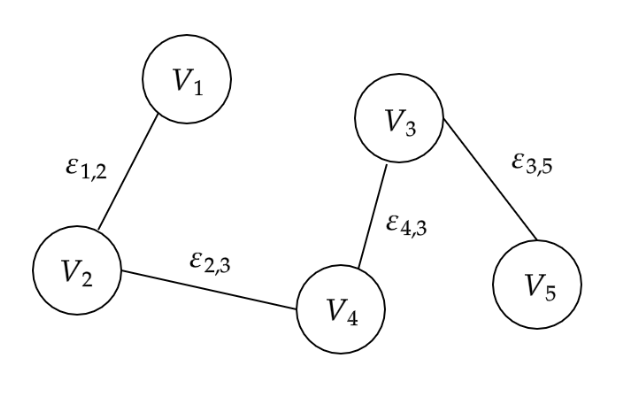
\includegraphics[width=0.4\linewidth]{Images/clustering/Grafo.png}
    \caption{Esempio di grafo orientato.}
\end{figure}

L'obiettivo è trovare un taglio che divida il grafo in due cluster, il nostro obiettivo è trovare il taglio migliore. Per farlo è utile conoscere:
\begin{itemize}
  \item \textbf{Prodotto scalare e funzione reale vertici} $f : V \rightarrow \mathbb{R}$. Dato un vettore $f(f_1, f_2, \cdots, f_n) \in \mathbb{R}^n$ con $n = \mid V \mid$:
    \[
        \langle f, g \rangle_{\mathcal{H}(V)} := \sum_{x_i \in V} f(x_i)g(x_i)
    \]
  \item \textbf{Prodotto scalare e funzione reale archi}, $F : E \rightarrow \mathbb{R}$. Dato un vettore $F(f_1, f_2, \cdots, f_n) \in \mathbb{R}^n$ con $n = \mid E \mid$:
    \[
      \langle F, G \rangle_{\mathcal{G}(E)} := \sum_{x_i, x_j \in E} F(x_i, x_j)G(x_i, x_j)
    \]
\end{itemize}

\subsection{Operatori}
\begin{defn}[Differenza Pesata]
  La differenza pesata (o derivata pesata sul grafo) di $f$ lungo un arco orientato $(x_i, x_j) \in E$ è:
  \[
    \partial_{x_j} f(x_i) := \sqrt{w(x_i, x_j)} (f(x_j) - f(x_i))
  \]
\end{defn}

\begin{defn}[Gradiente Pesato]
  Sulla base della nozione di differenze pesate, si definisce l'operatore gradiente pesato sui grafi:
  \[
    \nabla_w : \mathcal{H}(V) \rightarrow \mathcal{H}(E)\nabla_w : \mathcal{H}(V) \rightarrow \mathcal{H}(E)
  \]
  Come:
  \[
    (\nabla_w f)(x_i, x_j) = \partial_{x_j} f(x_i)
  \]
\end{defn}

\begin{defn}[Adjoint]
  Due operatori, si definiscono adjoin, quando si possono invertire l’ordine dell’operazione, per invertire l’operatore desiderato.
  L'operatore adjoint $\nabla_w^* : \mathcal{H}(E) \rightarrow \mathcal{H}(V)\nabla_w^* : \mathcal{H}(E) \rightarrow \mathcal{H}(V)$ del gradiente pesato è un operatore lineare definito da:
  \[
    \langle \nabla_w f, G \rangle_{\mathcal{H}(E)} = \langle f, \nabla_w^* G \rangle_{\mathcal{H}(V)} \quad \forall f \in \mathcal{H}(V), G \in \mathcal{H}(E)
  \]
  Afficnhè:
  \[
    (\nabla_w^* F)(x_i) = \sum_{x_j \sim x_i} \sqrt{w(x_i, x_j)}(F(x_j, x_i) - F(x_i, x_j))
  \]
  L'operatore adjoint negativo $-\nabla_w^*$ è chiamato \textbf{divergenza}, che misura il flusso netto in uscita di una funzione di arco in ciascun vertice del grafo.
\end{defn}

\begin{defn}[Laplaciano]
  È un operatore utile, per il calcolo del taglio ottimo, si ottiene facendo la divergenza del gradiente di una funzione:
  \[
    (\text{div}_w(\nabla_w f))(x_i)
  \]
\end{defn}
\newpage
Dato un grafo, possiamo ottenere il laplaciano in questo modo:
\[
 L = D - W
\]
Dove:
\begin{itemize}
  \item \textbf{W} è una matrice $i \times j$ con $w_{ij}$ è il peso che collega $i$ e $j$.
  \item \textbf{D} è una matrice diagonale, in cui nella diagonale ha la somma della riga.
\end{itemize}

\section{Partizione Dati tramite Grafi}
Dato un dataset $D = \{x_i\}^N_{i = 1}$ con $x_i \in \mathcal{R}^D$, possiamo costruire un grafo nel quale:
\begin{itemize}
  \item Ogni vertice $V$ è un datapoint $V_i = x_i$.
  \item Il peso di ogni arco $w_{ij}$ è la similiarità fra i due datapoint $(V_i, V_j) = (x_i, x_j)$.
\end{itemize}

\subsection{Bi-Partizione del Grafo}
Per ottenere due insieme di vertici disgiunti bisogna tagliare gli archi che li connettono, avendo un costo:
\[
  \text{CUT}(A, B) = \sum_{i \in A, j \in B}{w_{ij}}
\]
Ossia, la sommatoria della somiglianza tra gli oggetti dei due cluster.

\begin{figure}[!htb]
    \centering
    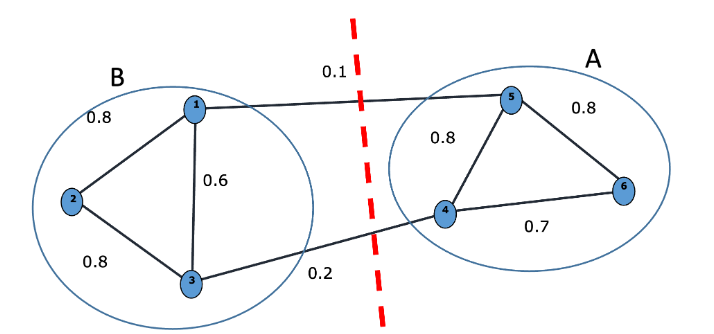
\includegraphics[width=0.5\linewidth]{Images/clustering/Grafo_cut.png}
    \caption{Esempio di bi-partizionamento di un grafo.}
\end{figure}

Esistono due approcci di clustering dei grafi:
\begin{enumerate}
  \item \textbf{Minimum cut:} $\text{mincut}(A, B)$.
  \item \textbf{Normalized cut:} $\text{minNcut}(A, B) = \frac{\text{cut}(A, B)}{vol(A)} + \frac{\text{cut}(A, B)}{vol(B)}$.
\end{enumerate}

\subsection{Minimum Cut}
Risolvere il problema del taglio minimo equivale a trovare un vettore discreto $p$ dove:
\[
  p = \begin{cases} +1 \text{ se } V_i \in A \\ -1 \text{ se } V_i \in B \end{cases}
\]
è un problema NP completo.
Possiamo per risolverlo usando $f : V \rightarrow R$ come rilassamento di $p$. \\
Riscrivendo l'equazione otteniamo:
\[
  \text{mincut}(A, B) \arg\min_f \sum_E w_{i,j}(f_i - f_j)^2
\]
O in forma matriciale:
\[
  f^TLf
\]
Che equivale anche all'\textbf{Energia di Dirichlet}, usata per calcolare la regolarità di una funzione:
\[
  \sum_E \|\nabla_w f\|^2
\]
\begin{note}[Ottimizzazione]
  Risolvere i problemi di taglio minimo equivale a trovare un campo di vertici continuo $f$ che minimizzi $f^TLf$ che equivale a minimizzare l'energia di Dirichlet.
\end{note}

\begin{thm}[Teorema di Rayleigh]
  La soluzione Mincut $f^*$ è:
  \begin{itemize}
    \item Il secondo autovettore più piccolo di $L$.
    \item Il valore di taglio è il secondo autovalore più piccolo di $L$.
  \end{itemize}
  Tutte le possibili soluzioni non sovrapposte di $\arg\min_f \sum_E \|\nabla_w f\|^2$ equivalgono agli autovettori del laplaciano $L$ ordinati per autovalori crescenti.
\end{thm}

Infine, per partizionare un grafo in $k$ cluster, posso usare ricorsivamente la tecnica del bi-partizionamento.
